\begin{frame}
\frametitle{There is more than just classification}
\begin{columns}[c]
\column{.4\textwidth}
\begin{itemize}
\item Canonical Correlation Analysis
\item Multi-Way, Multi-View Learning
\item Other existing methods
\item Methods not yet invented
\end{itemize}
\column{.6\textwidth}
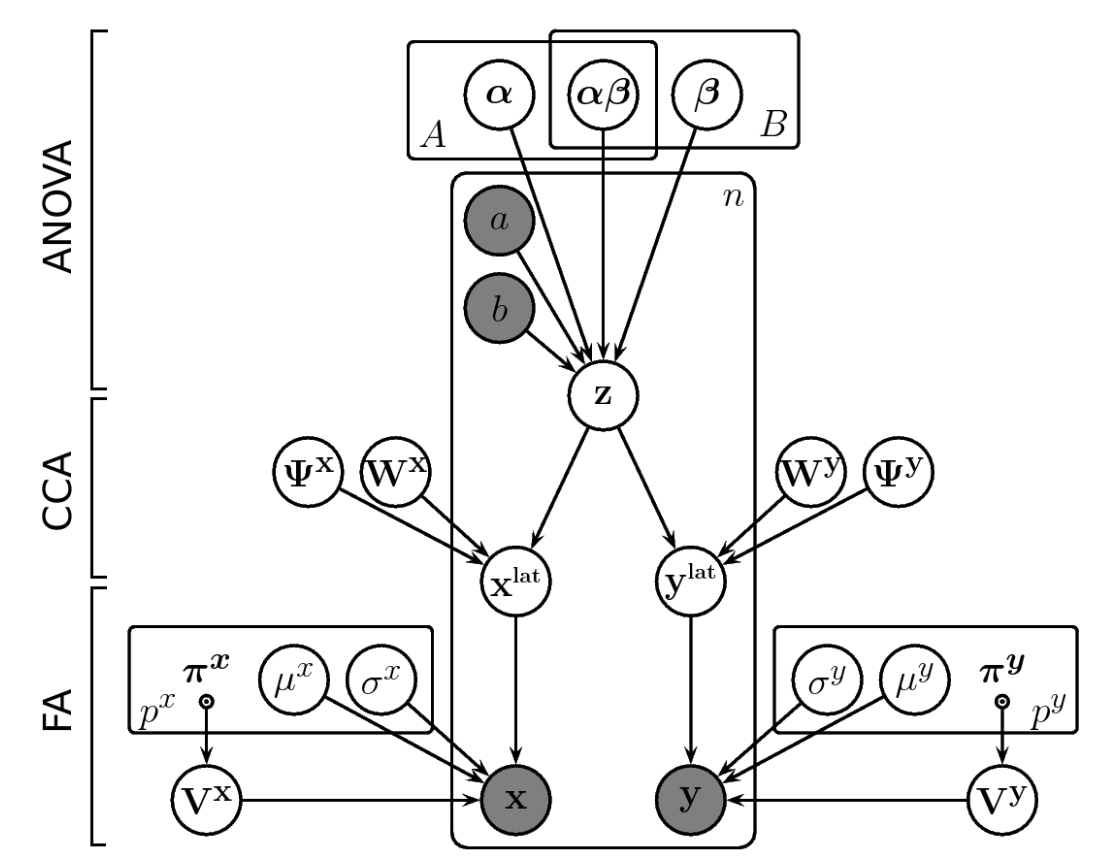
\includegraphics[width=\textwidth]{huopaniemi}

{\itshape\tiny Huopaniemi, Ilkka, Tommi Suvitaival, Janne Nikkil\"{a}, Matej Ore\v{s}i\v{c}, and Samuel Kaski. ``Multi-way, multi-view learning.'' arXiv preprint arXiv:0912.3211 (2009).\par}
\end{columns}
\end{frame}


\begin{frame}
\frametitle{Kernel Matrices}
Linear kernel matrices may computed from the raw features.
\begin{eqnarray*}
{\bf C} = {\bf V}{\bf V}^T
\end{eqnarray*}
A simple spatial feature selection may be considered as the following, where ${\bf A}$ is a diagonal matrix of ones and zeros:
\begin{eqnarray*}
{\bf C} = {\bf V}{\bf A}{\bf V}^T
\end{eqnarray*}
However, ${\bf A}$ may be more complicated, for example encoding spatial smoothing, high-pass filtering or any number of other things.
\end{frame}

\begin{frame}
\frametitle{Inner Products}
This gives us an alternative way of measuring distances between vectors in a linear way, where ${\bf A}$ is symmetric and positive definite.
\begin{eqnarray*}
d({\bf v}_1,{\bf v}_2) = \sqrt{({\bf v}_1 - {\bf v}_2)^T {\bf A} ({\bf v}_1 - {\bf v}_2)}
\end{eqnarray*}

Usually, the operation ${\bf A}{\bf v}^T$ is performed as a convolution.  For example, when dealing with 2D data, we may convolve with the Laplacian operator.
\begin{eqnarray*}
{\nabla}^2 {\bf v} = {\bf v} \ast \begin{pmatrix} 0 & -1 & 0\cr -1 & 4 & -1\cr 0 & -1 & 0\end{pmatrix}
\end{eqnarray*}

Note that the actual form of ${\bf A}$ can vary, so we need to figure out what metric tensor is optimal.
\end{frame}

